\vspace{5 mm}  %to enter vertical space
\subsection{Lets Create a Yard}
\vspace{2mm}
\subsubsection*{\underline{Preparing for drawing:}}
\begin{itemize}
\item{\textbf{Setting the Units:} Goto to Edit menu $>$ Current Drawing Preference, goto Tab \textbf{Unit} $>$ select \textbf{Inch} as main Drawing units. Also select \textbf{Archtectural} as a Format of unit.
       \begin{figure}[h!]
       \centering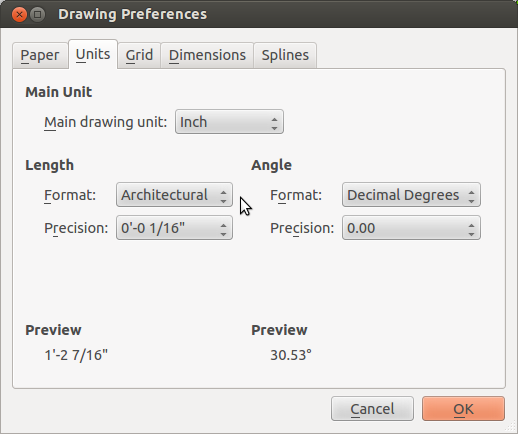
\includegraphics[width=220px]{./images-yard/units.png}
       \caption{\small \sl Setting Units for Yard}
       \end{figure}}
\item{\textbf{Turning ON Grid:} Goto to Edit menu $>$ Current Drawing Preference, goto Tab \textbf{Grid} $>$ check the \textbf{Show Grid} Option $>$ select \textbf{Orthogonal Grid}.
       \begin{figure}[h!]
       \centering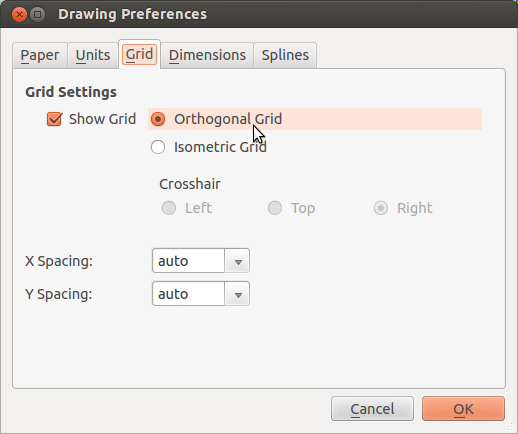
\includegraphics[width=220px]{./images-yard/grid.png}
       \caption{\small \sl Setting Grid for Yard}
       \end{figure}}
\item{\textbf{Turning ON Snap:} Goto Snap menu $>$ select \textbf{Snap on Grdi} for an instance. Snapping will be choosen to find accurate position according to the situation.
\begin{figure}[h!]
       \centering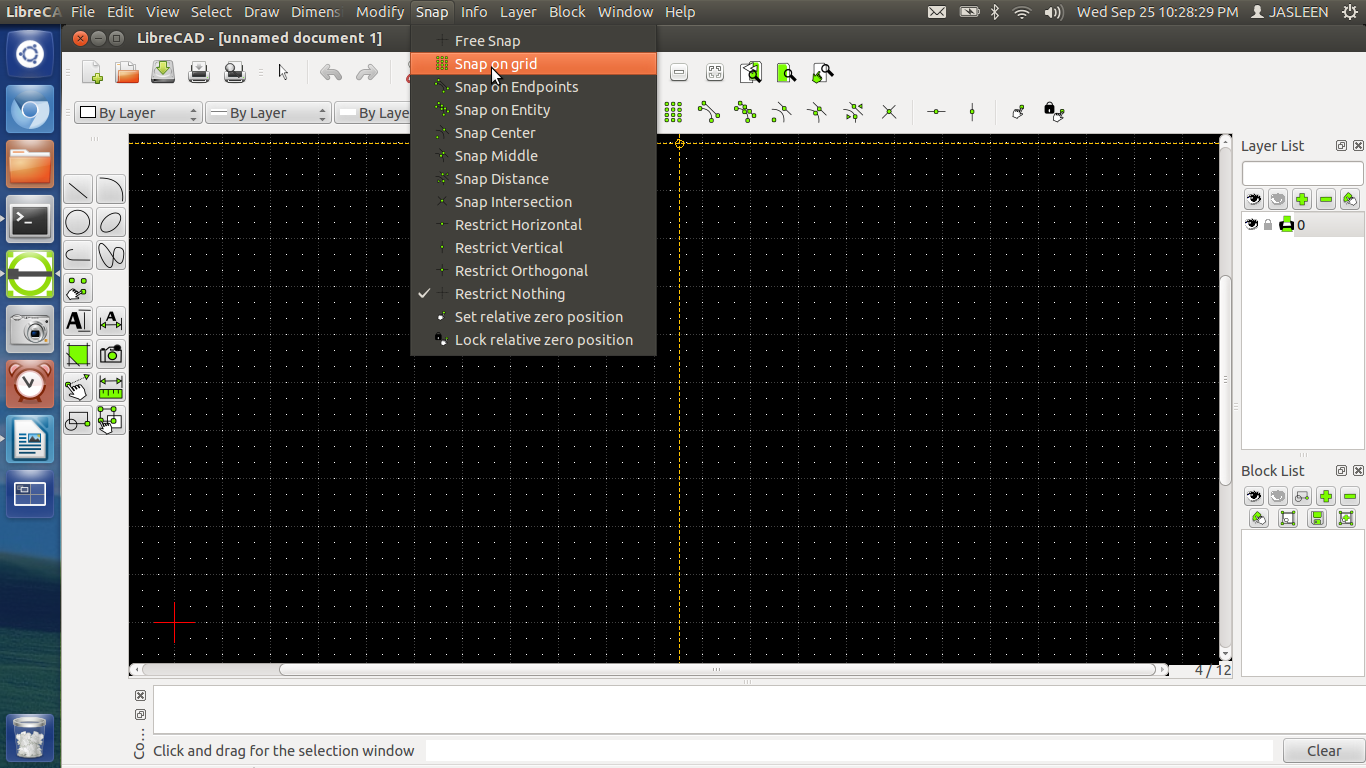
\includegraphics[width=400px]{./images-yard/snap.png}
       \caption{\small \sl Setting Grid for Yard}
       \end{figure}}
\end{itemize}\vspace{5mm}
%
\subsubsection*{\underline{Creating Layers:}}
On the Right side of screen, there is a \textbf{Layer List}, which is used to add/edit layers. Create a new Layer with $+$ icon. Add name of Layer and select its attributes.
\\Create these layers for Yard Drawing with following Colors and LineType.
       \begin{figure}[h!]
       \centering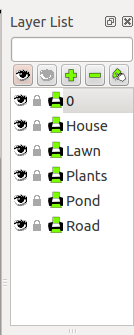
\includegraphics[width=60px]{./images-yard/layers.png}
       \caption{\small \sl Creating Layers}
       \end{figure}
\begin{table}[h!]\centering\begin{tabular}{|c|c|c|}
\hline \textbf{Name} & \textbf{Color} & \textbf{Line Type}\\ 
\hline House & White & Continous\\
\hline Lawn & Magenta & Continous\\
\hline Lot & Blue & Dash\\
\hline Plant & Green & Continous\\
\hline Pond & Cyan & Continous\\
\hline Road & Red & Continous\\
\hline Dimension & others(pink) & Continous\\
\hline \end{tabular}\end{table} 
\vspace{.3in}
%
\subsubsection*{\underline{Save the Drawing:}}
Now you can save your Drawing. Goto \textbf{File} menu $>$ \textbf{Save as.}
%
\newpage
\vspace{3mm}
\subsection*{\underline{Start Creating Drawing:}}\vspace{.5in}
\begin{enumerate}
\item{Make the \textbf{Lot} Layer active to Drawing Area, from Layer List.}
\item{Start Drawing with Line. Type `li' (shorthand for line) in Command Line. It will promp you:
\begin{verbatim}
Specify First point: 40,40
Specify next Point: @116<0
Specify next Point: @80<90
Specify next Point: @76<180
Specify next Point: @50<216.88
Specify next Point: @40,40
\end{verbatim}
Single \textbf{Right Click} is used to come out of \textbf{Line} Command. 
Here points are given as polar coordinates or cartesian coordinates\\
\textbf{(40,40)} is a cartesian coordinate, which (x,y) point with respect to absolute value(0,0).\\
\textbf{@116$<$0} is a polar coordinate, where, `@' is to use Relative cordinates, '116' is Distance in inch from previous end point, "$<$'is to draw angle, '0' is the degree of angle by line is drawn.\\\\
\begin{figure}[h!]
       \centering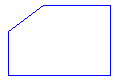
\includegraphics[width=180px]{./images-yard/lot.png}
       \caption{\small \sl Creating Lot of yard Drawing}
       \end{figure}
\\Now \textbf{Lot} is created, save your drawing as -  File $>$ Save.}
%
\item{Make the \textbf{House} Layer active to Drawing Area, from Layer List.}
\item{Select polyline entity by typing \textbf{polyline} in a Command Line.\\
Turn on \textbf{Snap on end point.}
\begin{verbatim}
Specify First point: <Pick lower Right corner of 'Lot' using snap on endpoint>
Specify next Point: @30<90
Specify next Point: @3<0
Specify next Point: @20<90
Specify next Point: @28<180
Specify next Point: @50<270
Specify next Point: <Pick lower Right corner of 'Lot' using snap on endpoint>
then right click to leave the polyline command.
\end{verbatim}
\begin{figure}[h!]
       \centering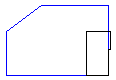
\includegraphics[width=180px]{./images-yard/house-rt.png}
       \caption{\small \sl Creating House of yard Drawing}
       \end{figure}
Use \textbf{Move} Command from \textbf{Modify} Menu, to move the House.
\begin{verbatim}
Specify to move: <Pick any point of house, whole house will be selected as one entity>
Specify Reference Point: <Pick any lower left corner of house>
Specify Target Point: @10<90
\end{verbatim} 
Again use Move Command.
\begin{verbatim}
Specify to move: <Pick any point of house, whole house will be selected as one entity>
Specify Reference Point: <Pick any lower left corner of house>
Specify Target Point: @20<-180
\end{verbatim} 
\begin{figure}[h!]
       \centering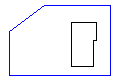
\includegraphics[width=180px]{./images-yard/house-mv.png}
       \caption{\small \sl Moving House to its position}
       \end{figure}
Now \textbf{House} is created, again save your drawing as -  File $>$ Save.}
%
\item{Make the \textbf{Road} Layer active}
\item{Select polyline.
\begin{verbatim}
Specify First point: <Pick upper Right corner of 'House' using Snap on Endpoint>
Specify next Point: @28<0
Specify next Point: @40<90
then right click to leave the polyline command.
\end{verbatim}
Select the Round Option from Modify menu, to round the turn of Road. Select the radius of round curve as 10.0 and also check the trim option to trim the intersecion of two lines.

\includegraphics[width=80px]{./images-yard/round.png}
\begin{figure}[h!]
       \centering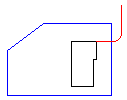
\includegraphics[width=160px]{./images-yard/round-c.png}
       \caption{\small \sl Creating one side of Road}
       \end{figure}
\\As one side of Road is created. Now create other side of road usinf Mirror command.
\\Turn ON snap on Entity, Middle, Distance.
\\Goto Modify $>$ Mirror.
\begin{verbatim}
Select the Entity: < select road>
Specify first point of Mirror Line:<pick a point vertical to house's left edge on right side>
Specify second point of Mirror Line:<pick a point vertical to house' left edge on left side>
\end{verbatim}
A mirror image appears in preview, set its angle by moving your cursor and then hit click to stay on that preview. A dialog box will open , select 'keep original'and then click OK.
\begin{figure}[h!]
       \centering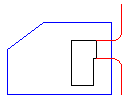
\includegraphics[width=160px]{./images-yard/road.png}
       \caption{\small \sl Creating other side of Road}
       \end{figure}
       Note: You can UNDO your mistake anytime.}
\item{Make the \textbf{Lawn} Layer active}
\item{Select Spline. Then select the middle of Lot (Diagonal side), using snap on Middle and Intersection. Click on middle point, then using Free snap, make a free-hand line with continuous clicks till it reach the other side of Lot.
\\Then selecting polyline and using Snap on Endpoint, cover the whole Lawn. Make sure to Lock all other Layers. So that you can easily pick point of your Lawn Layer. Locking a Layer is useful to select the objects overlaying on different layers. Locking makes the layer visible, but you cant pick that Locked Layer.
\begin{figure}[h!]
       \centering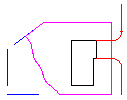
\includegraphics[width=180px]{./images-yard/lawn-full.png}
       \caption{\small \sl Lawn of Yard Drawing}
       \end{figure}
You can save your drawing now.}
\item{Make the \textbf{Plant} Layer active}
\item{Create a Block in a seperate drawing document and then import it in you drawing. Block is useful when we have to draw same thing at many places, with same/different scaling factor. Using Block we create the thing once, and used that block many times.\\
TO create a Block of Tree, First make a circle, and then a line crossing from its center (using Snap on Center) and coming smaller towards the outer of circle boundary. Now goto Modify menu $>$ Rotate. 
\begin{verbatim}
Select the Entity to rotate: <select line in circle>
Click on run.
Specify Rotation center: <select center of circle>
Specify Reference point: <select center of circle>
Specify Target point: <select center of circle>
\end{verbatim}
\vspace{.2in}
\begin{figure}[h!]
       \centering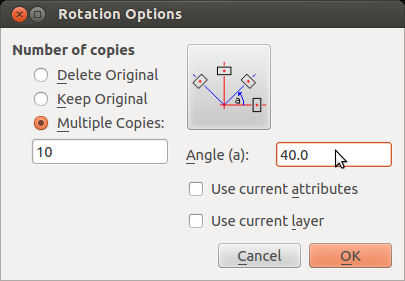
\includegraphics[width=210px]{./images-yard/rotate.png}
       \caption{\small \sl Rotate Dialogue box}
       \end{figure}
       \vspace{.5in}
       Set the rotate angle at 40 degree and keep multiple copies. A tree will be created.\\
Click on create Block option from Block menu. Select tree as whole entity to create a block.\\
click on run 
\includegraphics[width=40px]{./images-yard/run.png}\\
select reference point say (0,0)\\
Adialog box will appear, enter name of your Block (Tree). the click ok. A box will be created and will listed on Block List which is on right side below the layer List.\\
Goto Block menu $>$ Save your block as a seprate document. 
Now, you can insert this block wherever you want.
\\\\
To insert the block to your drawing. Open your drawing. Goto to File menu $>$ Import $>$ Block. Browse you block from your system. when you opened it, you will see the block appears in Block List.\\
Click on insert icon on Block List.\\
Specify any point as a reference point.\\
click on run.\\
insert the block where ever you want. you can scale your block by writting scale factor in box whick appears suring block command. or You can scale from Modify menu $>$ Scale.\\
Insert the tree block where you want on different scales.\\
\begin{figure}[h!]
       \centering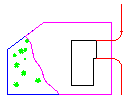
\includegraphics[width=180px]{./images-yard/tree.png}
       \caption{\small \sl Inserted Tree blocks in Plant Layer}
       \end{figure}}
\item{Make the \textbf{Dimension} Layer active. Create pond using Ellipse.}
\item{Make the \textbf{Fence} Layer active}
\item{Select Polyline to draw Fence. Here snapping will be trickly most used. 
\begin{verbatim}
Specify First point: <Pick middle 'House' using Snap on Middle and snap on Entity>
Specify next Point: <To select next point, Restrict vertical and on Entity>
Specify next Point: <Now unselect Restrict Veritcal and select snap on Endpoint>
Specify next Point: <select point using snap on Endpoint>
Specify next Point: <select point using snap on Endpoint>
Specify next Point: <select point using snap on Endpoint>
Specify next Point: <select point by selecting Restrict Orthogonaly, select the point by matching Crosshairs with the first line you created with same command>
Specify next Point: <select last point using snap on Entity>
then right click to leave the polyline command.
\end{verbatim}
\begin{figure}[h!]
       \centering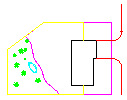
\includegraphics[width=180px]{./images-yard/fense.png}
       \caption{\small \sl Fense in yard}
       \end{figure}}    
\item{Make the \textbf{Dimension} Layer active\\
In Dimension Layer, we will add Text and Dimensions both at same layer.\\
To add Text, Goto Draw menu $>$ Text. A dialogue box will appear, Enter your text, select the Height of text and angle by which you rotate text. then click OK. Place your text in drawing area where you want.\\
To add Dimensions, goto Dimension Menu, select type of dimension. I used Vertical, Horizonal, alligned dimensions in my drawing and also Leder to indicate some part of Drawing.
\begin{figure}[h!]
       \centering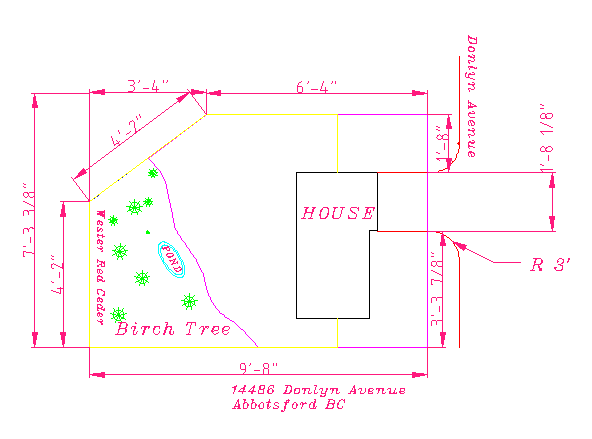
\includegraphics[width=380px]{./images-yard/dimension.png}
       \caption{\small \sl Drawing of Yard with Dimensioning}
       \end{figure}
\newpage
\large{The complete Drawing of Yard:}      
\begin{figure}[h!]
       \centering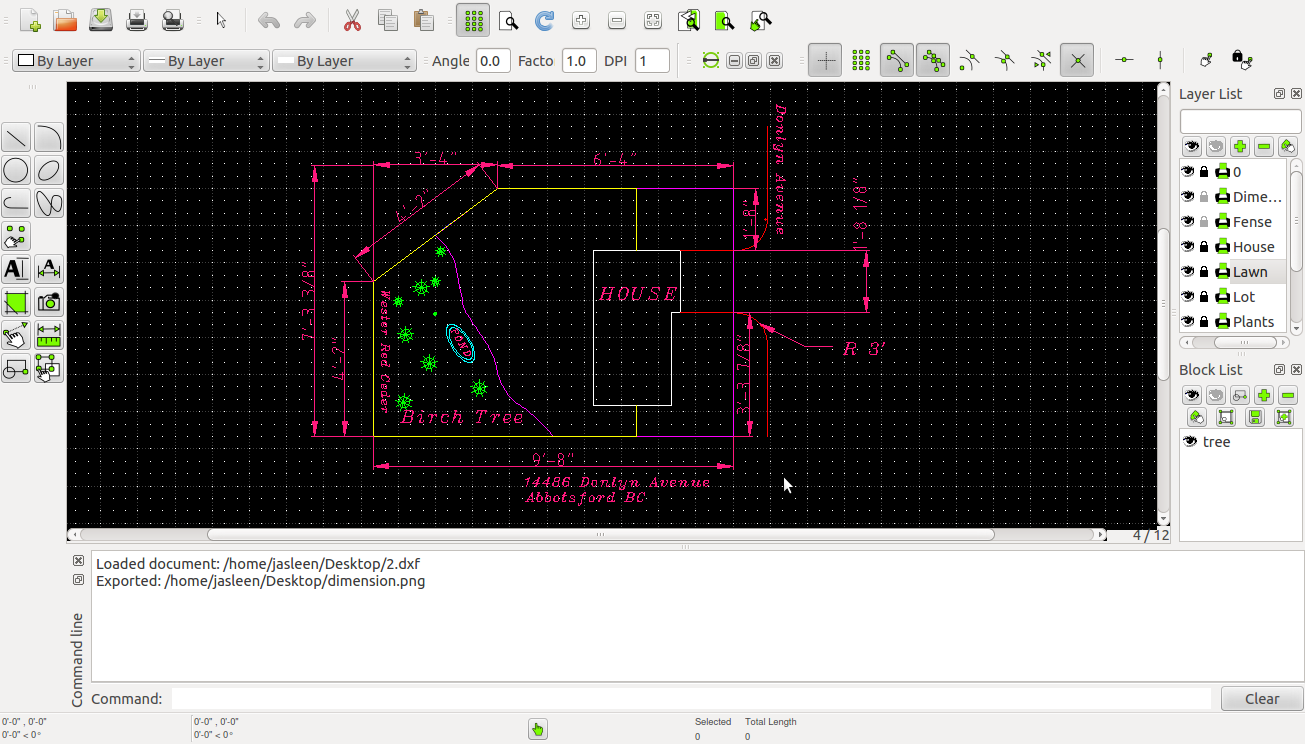
\includegraphics[width=450px]{./images-yard/complete.png}
       \caption{\small \sl Drawing of Yard with Dimensioning}
       \end{figure}}
\end{enumerate}
